\documentclass[twoside]{book}

% Packages required by doxygen
\usepackage{fixltx2e}
\usepackage{calc}
\usepackage{doxygen}
\usepackage[export]{adjustbox} % also loads graphicx
\usepackage{graphicx}
\usepackage[utf8]{inputenc}
\usepackage{makeidx}
\usepackage{multicol}
\usepackage{multirow}
\PassOptionsToPackage{warn}{textcomp}
\usepackage{textcomp}
\usepackage[nointegrals]{wasysym}
\usepackage[table]{xcolor}

% Font selection
\usepackage[T1]{fontenc}
\usepackage[scaled=.90]{helvet}
\usepackage{courier}
\usepackage{amssymb}
\usepackage{sectsty}
\renewcommand{\familydefault}{\sfdefault}
\allsectionsfont{%
  \fontseries{bc}\selectfont%
  \color{darkgray}%
}
\renewcommand{\DoxyLabelFont}{%
  \fontseries{bc}\selectfont%
  \color{darkgray}%
}
\newcommand{\+}{\discretionary{\mbox{\scriptsize$\hookleftarrow$}}{}{}}

% Page & text layout
\usepackage{geometry}
\geometry{%
  a4paper,%
  top=2.5cm,%
  bottom=2.5cm,%
  left=2.5cm,%
  right=2.5cm%
}
\tolerance=750
\hfuzz=15pt
\hbadness=750
\setlength{\emergencystretch}{15pt}
\setlength{\parindent}{0cm}
\setlength{\parskip}{3ex plus 2ex minus 2ex}
\makeatletter
\renewcommand{\paragraph}{%
  \@startsection{paragraph}{4}{0ex}{-1.0ex}{1.0ex}{%
    \normalfont\normalsize\bfseries\SS@parafont%
  }%
}
\renewcommand{\subparagraph}{%
  \@startsection{subparagraph}{5}{0ex}{-1.0ex}{1.0ex}{%
    \normalfont\normalsize\bfseries\SS@subparafont%
  }%
}
\makeatother

% Headers & footers
\usepackage{fancyhdr}
\pagestyle{fancyplain}
\fancyhead[LE]{\fancyplain{}{\bfseries\thepage}}
\fancyhead[CE]{\fancyplain{}{}}
\fancyhead[RE]{\fancyplain{}{\bfseries\leftmark}}
\fancyhead[LO]{\fancyplain{}{\bfseries\rightmark}}
\fancyhead[CO]{\fancyplain{}{}}
\fancyhead[RO]{\fancyplain{}{\bfseries\thepage}}
\fancyfoot[LE]{\fancyplain{}{}}
\fancyfoot[CE]{\fancyplain{}{}}
\fancyfoot[RE]{\fancyplain{}{\bfseries\scriptsize Generated by Doxygen }}
\fancyfoot[LO]{\fancyplain{}{\bfseries\scriptsize Generated by Doxygen }}
\fancyfoot[CO]{\fancyplain{}{}}
\fancyfoot[RO]{\fancyplain{}{}}
\renewcommand{\footrulewidth}{0.4pt}
\renewcommand{\chaptermark}[1]{%
  \markboth{#1}{}%
}
\renewcommand{\sectionmark}[1]{%
  \markright{\thesection\ #1}%
}

% Indices & bibliography
\usepackage{natbib}
\usepackage[titles]{tocloft}
\setcounter{tocdepth}{3}
\setcounter{secnumdepth}{5}
\makeindex

% Hyperlinks (required, but should be loaded last)
\usepackage{ifpdf}
\ifpdf
  \usepackage[pdftex,pagebackref=true]{hyperref}
\else
  \usepackage[ps2pdf,pagebackref=true]{hyperref}
\fi
\hypersetup{%
  colorlinks=true,%
  linkcolor=blue,%
  citecolor=blue,%
  unicode%
}

% Custom commands
\newcommand{\clearemptydoublepage}{%
  \newpage{\pagestyle{empty}\cleardoublepage}%
}

\usepackage{caption}
\captionsetup{labelsep=space,justification=centering,font={bf},singlelinecheck=off,skip=4pt,position=top}

%===== C O N T E N T S =====

\begin{document}

% Titlepage & ToC
\hypersetup{pageanchor=false,
             bookmarksnumbered=true,
             pdfencoding=unicode
            }
\pagenumbering{alph}
\begin{titlepage}
\vspace*{7cm}
\begin{center}%
{\Large Projeto segunda unidade \\[1ex]\large \#finnished }\\
\vspace*{1cm}
{\large Generated by Doxygen 1.8.14}\\
\end{center}
\end{titlepage}
\clearemptydoublepage
\pagenumbering{roman}
\tableofcontents
\clearemptydoublepage
\pagenumbering{arabic}
\hypersetup{pageanchor=true}

%--- Begin generated contents ---
\chapter{D\+C\+A1202-\/}
\label{md__r_e_a_d_m_e}
\Hypertarget{md__r_e_a_d_m_e}
Projeto 1 -\/ Tratamento de polígonos 
\chapter{Hierarchical Index}
\section{Class Hierarchy}
This inheritance list is sorted roughly, but not completely, alphabetically\+:\begin{DoxyCompactList}
\item \contentsline{section}{Point}{\pageref{class_point}}{}
\item \contentsline{section}{Poligono}{\pageref{class_poligono}}{}
\begin{DoxyCompactList}
\item \contentsline{section}{Retangulo}{\pageref{class_retangulo}}{}
\end{DoxyCompactList}
\end{DoxyCompactList}

\chapter{Class Index}
\section{Class List}
Here are the classes, structs, unions and interfaces with brief descriptions\+:\begin{DoxyCompactList}
\item\contentsline{section}{\mbox{\hyperlink{class_point}{Point}} \\*A classe \mbox{\hyperlink{class_point}{Point}} serve para representar pontos no espaço bidimensional }{\pageref{class_point}}{}
\item\contentsline{section}{\mbox{\hyperlink{class_poligono}{Poligono}} \\*A classe \mbox{\hyperlink{class_poligono}{Poligono}} serve para representar os pontos do polígono no espaço bidimensional }{\pageref{class_poligono}}{}
\item\contentsline{section}{\mbox{\hyperlink{class_retangulo}{Retangulo}} \\*A classe \mbox{\hyperlink{class_retangulo}{Retangulo}} serve para representar os pontos do retangulo no espaço bidimensional }{\pageref{class_retangulo}}{}
\end{DoxyCompactList}

\chapter{Class Documentation}
\hypertarget{class_point}{}\section{Point Class Reference}
\label{class_point}\index{Point@{Point}}


A classe \mbox{\hyperlink{class_point}{Point}} serve para representar pontos no espaço bidimensional.  




{\ttfamily \#include $<$point.\+h$>$}

\subsection*{Public Member Functions}
\begin{DoxyCompactItemize}
\item 
\mbox{\Hypertarget{class_point_ad92f2337b839a94ce97dcdb439b4325a}\label{class_point_ad92f2337b839a94ce97dcdb439b4325a}} 
\mbox{\hyperlink{class_point_ad92f2337b839a94ce97dcdb439b4325a}{Point}} ()
\begin{DoxyCompactList}\small\item\em \mbox{\hyperlink{class_point}{Point}} é o construtor da classe. \end{DoxyCompactList}\item 
void \mbox{\hyperlink{class_point_a428a1676e2fdec6753c42011a1d59d18}{setX}} (float \+\_\+x)
\begin{DoxyCompactList}\small\item\em setX\+: Define o valor da coordenada x do ponto. \end{DoxyCompactList}\item 
void \mbox{\hyperlink{class_point_a9868c4601b0ea0c2d0de20fe41ee0e49}{setY}} (float \+\_\+y)
\begin{DoxyCompactList}\small\item\em setY\+: Define o valor da coordenada y do ponto. \end{DoxyCompactList}\item 
void \mbox{\hyperlink{class_point_ab5385c6d9bfa841e641e4709fc9f14cc}{set\+XY}} (float \+\_\+x, float \+\_\+y)
\begin{DoxyCompactList}\small\item\em set\+XY\+: Define o valor da coordenada x e y do ponto. \end{DoxyCompactList}\item 
\mbox{\Hypertarget{class_point_a9aa94b8fd07296e64d304ef3750db113}\label{class_point_a9aa94b8fd07296e64d304ef3750db113}} 
float \mbox{\hyperlink{class_point_a9aa94b8fd07296e64d304ef3750db113}{getX}} (void)
\begin{DoxyCompactList}\small\item\em getX\+: Recupera o valor da coordenada x do ponto. \end{DoxyCompactList}\item 
\mbox{\Hypertarget{class_point_a2444daa96871c89614510bc4bfcd19ce}\label{class_point_a2444daa96871c89614510bc4bfcd19ce}} 
float \mbox{\hyperlink{class_point_a2444daa96871c89614510bc4bfcd19ce}{getY}} (void)
\begin{DoxyCompactList}\small\item\em getY\+: Recupera o valor da coordenada y do ponto. \end{DoxyCompactList}\item 
\mbox{\hyperlink{class_point}{Point}} \mbox{\hyperlink{class_point_a9dbea84b07b0a8ec3bbb9e58b3d15899}{add}} (\mbox{\hyperlink{class_point}{Point}} p1)
\begin{DoxyCompactList}\small\item\em add\+: Adiciona as coordenadas (x,y) do ponto com as coordenadas de um ponto P1(x1,y1) fornecido, armazenando o resultado (x+x1,y+y1) nas coordenadas de um novo ponto, que deverá ser retornado para o cliente da classe. \end{DoxyCompactList}\item 
\mbox{\hyperlink{class_point}{Point}} \mbox{\hyperlink{class_point_a9cf2c53b0a4e6282a6712824bb4e9b00}{sub}} (\mbox{\hyperlink{class_point}{Point}} p1)
\begin{DoxyCompactList}\small\item\em sub\+: Subtrai as coordenadas (x,y) do ponto com as coordenadas de um ponto P1(x1,y1) fornecido, armazenando o resultado (x-\/x1,y-\/y1) nas coordenadas de um novo ponto, que deverá ser retornado para o cliente da classe. \end{DoxyCompactList}\item 
float \mbox{\hyperlink{class_point_aa3005a9d97e2cb05624414973a214788}{norma}} (void)
\begin{DoxyCompactList}\small\item\em norma\+: Calcula a distância do ponto para a origem do sistema de coordenadas. \end{DoxyCompactList}\item 
void \mbox{\hyperlink{class_point_ad9676e36f3444534b609e3c68422239a}{translada}} (float a, float b)
\begin{DoxyCompactList}\small\item\em translada\+: Translada o ponto (x,y) de (+a,+b), de modo que, após a execução do método, as coordenadas do ponto serão (x+a,y+b). \end{DoxyCompactList}\item 
void \mbox{\hyperlink{class_point_a188350fb70e5b297a659a31ab8887ca3}{imprime}} (void)
\begin{DoxyCompactList}\small\item\em imprime\+: Imprime o ponto na forma (xpos, ypos). \end{DoxyCompactList}\end{DoxyCompactItemize}


\subsection{Detailed Description}
A classe \mbox{\hyperlink{class_point}{Point}} serve para representar pontos no espaço bidimensional. 

\subsection{Member Function Documentation}
\mbox{\Hypertarget{class_point_a9dbea84b07b0a8ec3bbb9e58b3d15899}\label{class_point_a9dbea84b07b0a8ec3bbb9e58b3d15899}} 
\index{Point@{Point}!add@{add}}
\index{add@{add}!Point@{Point}}
\subsubsection{\texorpdfstring{add()}{add()}}
{\footnotesize\ttfamily \mbox{\hyperlink{class_point}{Point}} Point\+::add (\begin{DoxyParamCaption}\item[{\mbox{\hyperlink{class_point}{Point}}}]{p1 }\end{DoxyParamCaption})}



add\+: Adiciona as coordenadas (x,y) do ponto com as coordenadas de um ponto P1(x1,y1) fornecido, armazenando o resultado (x+x1,y+y1) nas coordenadas de um novo ponto, que deverá ser retornado para o cliente da classe. 


\begin{DoxyParams}{Parameters}
{\em p1} & é um ponto atribuido pelo usuário. 
\begin{DoxyPre}
int main(void)\{
   \mbox{\hyperlink{class_point}{Point}} p1,p2,p3;
   p1.setXY(1,0);
   p2.setXY(9,1);
   p3 = p1.add(p2);
\}
\end{DoxyPre}
 \\
\hline
\end{DoxyParams}
\mbox{\Hypertarget{class_point_a188350fb70e5b297a659a31ab8887ca3}\label{class_point_a188350fb70e5b297a659a31ab8887ca3}} 
\index{Point@{Point}!imprime@{imprime}}
\index{imprime@{imprime}!Point@{Point}}
\subsubsection{\texorpdfstring{imprime()}{imprime()}}
{\footnotesize\ttfamily void Point\+::imprime (\begin{DoxyParamCaption}\item[{void}]{ }\end{DoxyParamCaption})}



imprime\+: Imprime o ponto na forma (xpos, ypos). 


\begin{DoxyPre}
int main(void)\{
   \mbox{\hyperlink{class_point}{Point}} p1;
   p1.setXY(6,9);
   p1.translada(1,4);
\}
\end{DoxyPre}
 \mbox{\Hypertarget{class_point_aa3005a9d97e2cb05624414973a214788}\label{class_point_aa3005a9d97e2cb05624414973a214788}} 
\index{Point@{Point}!norma@{norma}}
\index{norma@{norma}!Point@{Point}}
\subsubsection{\texorpdfstring{norma()}{norma()}}
{\footnotesize\ttfamily float Point\+::norma (\begin{DoxyParamCaption}\item[{void}]{ }\end{DoxyParamCaption})}



norma\+: Calcula a distância do ponto para a origem do sistema de coordenadas. 


\begin{DoxyParams}{Parameters}
{\em p1} & é um ponto atribuido pelo usuário. \\
\hline
\end{DoxyParams}
\mbox{\Hypertarget{class_point_a428a1676e2fdec6753c42011a1d59d18}\label{class_point_a428a1676e2fdec6753c42011a1d59d18}} 
\index{Point@{Point}!setX@{setX}}
\index{setX@{setX}!Point@{Point}}
\subsubsection{\texorpdfstring{set\+X()}{setX()}}
{\footnotesize\ttfamily void Point\+::setX (\begin{DoxyParamCaption}\item[{float}]{\+\_\+x }\end{DoxyParamCaption})}



setX\+: Define o valor da coordenada x do ponto. 


\begin{DoxyParams}{Parameters}
{\em \+\_\+x} & é o valor atribuido a coordenada. \\
\hline
\end{DoxyParams}
\mbox{\Hypertarget{class_point_ab5385c6d9bfa841e641e4709fc9f14cc}\label{class_point_ab5385c6d9bfa841e641e4709fc9f14cc}} 
\index{Point@{Point}!set\+XY@{set\+XY}}
\index{set\+XY@{set\+XY}!Point@{Point}}
\subsubsection{\texorpdfstring{set\+X\+Y()}{setXY()}}
{\footnotesize\ttfamily void Point\+::set\+XY (\begin{DoxyParamCaption}\item[{float}]{\+\_\+x,  }\item[{float}]{\+\_\+y }\end{DoxyParamCaption})}



set\+XY\+: Define o valor da coordenada x e y do ponto. 


\begin{DoxyParams}{Parameters}
{\em \+\_\+x} & e \+\_\+y é o valor atribuido aos pontos das coordenada. \\
\hline
\end{DoxyParams}
\mbox{\Hypertarget{class_point_a9868c4601b0ea0c2d0de20fe41ee0e49}\label{class_point_a9868c4601b0ea0c2d0de20fe41ee0e49}} 
\index{Point@{Point}!setY@{setY}}
\index{setY@{setY}!Point@{Point}}
\subsubsection{\texorpdfstring{set\+Y()}{setY()}}
{\footnotesize\ttfamily void Point\+::setY (\begin{DoxyParamCaption}\item[{float}]{\+\_\+y }\end{DoxyParamCaption})}



setY\+: Define o valor da coordenada y do ponto. 


\begin{DoxyParams}{Parameters}
{\em \+\_\+y} & é o valor atribuido a coordenada \\
\hline
\end{DoxyParams}
\mbox{\Hypertarget{class_point_a9cf2c53b0a4e6282a6712824bb4e9b00}\label{class_point_a9cf2c53b0a4e6282a6712824bb4e9b00}} 
\index{Point@{Point}!sub@{sub}}
\index{sub@{sub}!Point@{Point}}
\subsubsection{\texorpdfstring{sub()}{sub()}}
{\footnotesize\ttfamily \mbox{\hyperlink{class_point}{Point}} Point\+::sub (\begin{DoxyParamCaption}\item[{\mbox{\hyperlink{class_point}{Point}}}]{p1 }\end{DoxyParamCaption})}



sub\+: Subtrai as coordenadas (x,y) do ponto com as coordenadas de um ponto P1(x1,y1) fornecido, armazenando o resultado (x-\/x1,y-\/y1) nas coordenadas de um novo ponto, que deverá ser retornado para o cliente da classe. 


\begin{DoxyParams}{Parameters}
{\em p1} & é um ponto atribuido pelo usuário. 
\begin{DoxyPre}
int main(void)\{
   \mbox{\hyperlink{class_point}{Point}} p1,p2,p3;
   p1.setXY(1,0);
   p2.setXY(9,1);
   p3 = p1.sub(p2);
\}
\end{DoxyPre}
 \\
\hline
\end{DoxyParams}
\mbox{\Hypertarget{class_point_ad9676e36f3444534b609e3c68422239a}\label{class_point_ad9676e36f3444534b609e3c68422239a}} 
\index{Point@{Point}!translada@{translada}}
\index{translada@{translada}!Point@{Point}}
\subsubsection{\texorpdfstring{translada()}{translada()}}
{\footnotesize\ttfamily void Point\+::translada (\begin{DoxyParamCaption}\item[{float}]{a,  }\item[{float}]{b }\end{DoxyParamCaption})}



translada\+: Translada o ponto (x,y) de (+a,+b), de modo que, após a execução do método, as coordenadas do ponto serão (x+a,y+b). 


\begin{DoxyParams}{Parameters}
{\em a} & e b são valores atribuido pelo usuário. \\
\hline
\end{DoxyParams}


The documentation for this class was generated from the following files\+:\begin{DoxyCompactItemize}
\item 
point.\+h\item 
point.\+cpp\end{DoxyCompactItemize}

\hypertarget{class_poligono}{}\section{Poligono Class Reference}
\label{class_poligono}\index{Poligono@{Poligono}}


A classe \mbox{\hyperlink{class_poligono}{Poligono}} serve para representar os pontos do polígono no espaço bidimensional.  




{\ttfamily \#include $<$poligono.\+h$>$}

Inheritance diagram for Poligono\+:\begin{figure}[H]
\begin{center}
\leavevmode
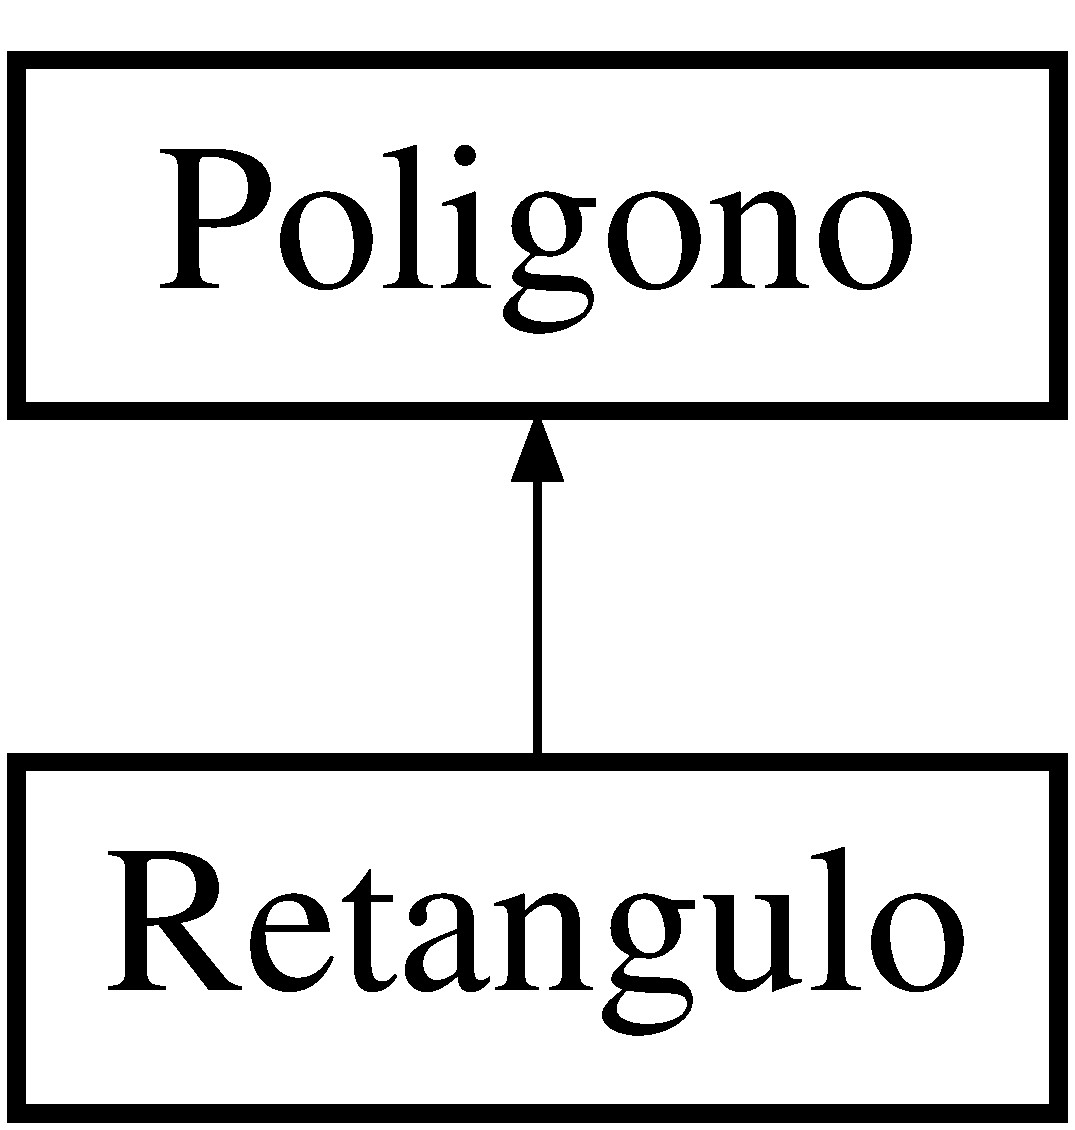
\includegraphics[height=2.000000cm]{class_poligono}
\end{center}
\end{figure}
\subsection*{Public Member Functions}
\begin{DoxyCompactItemize}
\item 
\mbox{\Hypertarget{class_poligono_a9311a9a1496878c09c8508b3636e2870}\label{class_poligono_a9311a9a1496878c09c8508b3636e2870}} 
\mbox{\hyperlink{class_poligono_a9311a9a1496878c09c8508b3636e2870}{Poligono}} ()
\begin{DoxyCompactList}\small\item\em \mbox{\hyperlink{class_poligono}{Poligono}} é o construtor da classe. \end{DoxyCompactList}\item 
void \mbox{\hyperlink{class_poligono_a9bd6496f563d349046c74e3b0f03ef19}{insert\+Pontos}} (\mbox{\hyperlink{class_point}{Point}} p)
\begin{DoxyCompactList}\small\item\em insert\+Pontos\+: Define os pontos do póligono. \end{DoxyCompactList}\item 
void \mbox{\hyperlink{class_poligono_a7db9753df6a913b910f3d293f6324267}{insert\+Pontos}} (float a, float b)
\begin{DoxyCompactList}\small\item\em insert\+Pontos\+: Define os pontos do póligono. \end{DoxyCompactList}\item 
\mbox{\Hypertarget{class_poligono_a9d011cabfeeeb85eae016cd2474b5e59}\label{class_poligono_a9d011cabfeeeb85eae016cd2474b5e59}} 
int \mbox{\hyperlink{class_poligono_a9d011cabfeeeb85eae016cd2474b5e59}{numerode\+Pontos}} ()
\begin{DoxyCompactList}\small\item\em numerode\+Pontos\+: Retorna o número de pontos do polígono. \end{DoxyCompactList}\item 
void \mbox{\hyperlink{class_poligono_a4d757f52ba9366ab13537fb19b363e1e}{translada\+Poligono}} (float a, float b)
\begin{DoxyCompactList}\small\item\em translada\+Poligono\+: Translada todos os pontos do polígono para (+a,+b), usando a funnção translada do ponto. \end{DoxyCompactList}\item 
\mbox{\Hypertarget{class_poligono_ac1e37e274f61dff6c421f972ef1cf891}\label{class_poligono_ac1e37e274f61dff6c421f972ef1cf891}} 
float \mbox{\hyperlink{class_poligono_ac1e37e274f61dff6c421f972ef1cf891}{area\+Poligono}} ()
\begin{DoxyCompactList}\small\item\em area\+Poligono\+: Retorna o valor da área do polígono. \end{DoxyCompactList}\item 
void \mbox{\hyperlink{class_poligono_ac187000d9b4ee9a33b193ae5d67f09ac}{rotacao\+Poligono}} (float angulo, \mbox{\hyperlink{class_point}{Point}} p)
\begin{DoxyCompactList}\small\item\em rotacao\+Poligono\+: Rotaciona o polígono de θ graus no sentido anti-\/horário em torno de um ponto (x0,y0) fornecido pelo usuário. \end{DoxyCompactList}\item 
void \mbox{\hyperlink{class_poligono_a16fcba48d87f60b030b61a54fd430fdd}{rotacao\+Poligono}} (float angulo, float x, float y)
\begin{DoxyCompactList}\small\item\em rotacao\+Poligono\+: Rotaciona o polígono de θ graus no sentido anti-\/horário em torno de um ponto (x0,y0) fornecido pelo usuário. \end{DoxyCompactList}\item 
float \mbox{\hyperlink{class_poligono_a61ad4f99fde11f7bb3077cd453152a95}{R\+C\+M\+Poligono}} (float angulo)
\begin{DoxyCompactList}\small\item\em R\+C\+M\+Poligono\+: Rotaciona o polígono de θ graus no sentido anti-\/horário em torno do centro de massa. \end{DoxyCompactList}\item 
\mbox{\Hypertarget{class_poligono_a824ada0183274d23180999c769947aaa}\label{class_poligono_a824ada0183274d23180999c769947aaa}} 
void \mbox{\hyperlink{class_poligono_a824ada0183274d23180999c769947aaa}{imprimir\+Poligono}} ()
\begin{DoxyCompactList}\small\item\em imprimir\+Poligono\+: Imprimir o polígono armazenado da forma (x0,y0)→(x1,y1)→(x2,y2)→…​ \end{DoxyCompactList}\end{DoxyCompactItemize}


\subsection{Detailed Description}
A classe \mbox{\hyperlink{class_poligono}{Poligono}} serve para representar os pontos do polígono no espaço bidimensional. 

\subsection{Member Function Documentation}
\mbox{\Hypertarget{class_poligono_a9bd6496f563d349046c74e3b0f03ef19}\label{class_poligono_a9bd6496f563d349046c74e3b0f03ef19}} 
\index{Poligono@{Poligono}!insert\+Pontos@{insert\+Pontos}}
\index{insert\+Pontos@{insert\+Pontos}!Poligono@{Poligono}}
\subsubsection{\texorpdfstring{insert\+Pontos()}{insertPontos()}\hspace{0.1cm}{\footnotesize\ttfamily [1/2]}}
{\footnotesize\ttfamily void Poligono\+::insert\+Pontos (\begin{DoxyParamCaption}\item[{\mbox{\hyperlink{class_point}{Point}}}]{p }\end{DoxyParamCaption})}



insert\+Pontos\+: Define os pontos do póligono. 


\begin{DoxyParams}{Parameters}
{\em p} & é o valor de um ponto atribuido ao póligono. 
\begin{DoxyPre}
int main(void)\{
// criacao de um poligono retangulo
   \mbox{\hyperlink{class_poligono}{Poligono}} a;
   \mbox{\hyperlink{class_point}{Point}} p1,p2,p3,p4;
   p1.setXY(0,0);
   p2.setXY(1,0);
   p1.setXY(1,1);
   p2.setXY(0,1);
   a.insertPontos(p1);
   a.insertPontos(p2);
   a.insertPontos(p3);
   a.insertPontos(p4);
\}
\end{DoxyPre}
 \\
\hline
\end{DoxyParams}
\mbox{\Hypertarget{class_poligono_a7db9753df6a913b910f3d293f6324267}\label{class_poligono_a7db9753df6a913b910f3d293f6324267}} 
\index{Poligono@{Poligono}!insert\+Pontos@{insert\+Pontos}}
\index{insert\+Pontos@{insert\+Pontos}!Poligono@{Poligono}}
\subsubsection{\texorpdfstring{insert\+Pontos()}{insertPontos()}\hspace{0.1cm}{\footnotesize\ttfamily [2/2]}}
{\footnotesize\ttfamily void Poligono\+::insert\+Pontos (\begin{DoxyParamCaption}\item[{float}]{a,  }\item[{float}]{b }\end{DoxyParamCaption})}



insert\+Pontos\+: Define os pontos do póligono. 


\begin{DoxyParams}{Parameters}
{\em a} & e b é o valor de um ponto atribuido ao póligono. 
\begin{DoxyPre}
int main(void)\{
// criacao de um poligono retangulo
   \mbox{\hyperlink{class_poligono}{Poligono}} a;
   a.insertPontos(0,0);
   a.insertPontos(1,0);
   a.insertPontos(1,1);
   a.insertPontos(0,1);
\}
\end{DoxyPre}
 \\
\hline
\end{DoxyParams}
\mbox{\Hypertarget{class_poligono_a61ad4f99fde11f7bb3077cd453152a95}\label{class_poligono_a61ad4f99fde11f7bb3077cd453152a95}} 
\index{Poligono@{Poligono}!R\+C\+M\+Poligono@{R\+C\+M\+Poligono}}
\index{R\+C\+M\+Poligono@{R\+C\+M\+Poligono}!Poligono@{Poligono}}
\subsubsection{\texorpdfstring{R\+C\+M\+Poligono()}{RCMPoligono()}}
{\footnotesize\ttfamily float Poligono\+::\+R\+C\+M\+Poligono (\begin{DoxyParamCaption}\item[{float}]{angulo }\end{DoxyParamCaption})}



R\+C\+M\+Poligono\+: Rotaciona o polígono de θ graus no sentido anti-\/horário em torno do centro de massa. 


\begin{DoxyParams}{Parameters}
{\em angulo} & é um valor atribuido pelo usuário. 
\begin{DoxyPre}
int main(void)\{
// criacao de um poligono retangulo
   \mbox{\hyperlink{class_poligono}{Poligono}} a;
   a.insertPontos(0,0);
   a.insertPontos(1,0);
   a.insertPontos(1,1);
   a.insertPontos(0,1);
   a.RMCPoligno(90);
\}
\end{DoxyPre}
 \\
\hline
\end{DoxyParams}
\mbox{\Hypertarget{class_poligono_ac187000d9b4ee9a33b193ae5d67f09ac}\label{class_poligono_ac187000d9b4ee9a33b193ae5d67f09ac}} 
\index{Poligono@{Poligono}!rotacao\+Poligono@{rotacao\+Poligono}}
\index{rotacao\+Poligono@{rotacao\+Poligono}!Poligono@{Poligono}}
\subsubsection{\texorpdfstring{rotacao\+Poligono()}{rotacaoPoligono()}\hspace{0.1cm}{\footnotesize\ttfamily [1/2]}}
{\footnotesize\ttfamily void Poligono\+::rotacao\+Poligono (\begin{DoxyParamCaption}\item[{float}]{angulo,  }\item[{\mbox{\hyperlink{class_point}{Point}}}]{p }\end{DoxyParamCaption})}



rotacao\+Poligono\+: Rotaciona o polígono de θ graus no sentido anti-\/horário em torno de um ponto (x0,y0) fornecido pelo usuário. 


\begin{DoxyParams}{Parameters}
{\em angulo} & e p são valores atribuido pelo usuário, ângulo e ponto de rotação. 
\begin{DoxyPre}
int main(void)\{
// criacao de um poligono retangulo
   \mbox{\hyperlink{class_poligono}{Poligono}} a;
   \mbox{\hyperlink{class_point}{Point}} p;
   a.insertPontos(0,0);
   a.insertPontos(1,0);
   a.insertPontos(1,1);
   a.insertPontos(0,1);
   p.setXY(0,0);
   a.rotacaoPoligno(90,p);
\}
\end{DoxyPre}
 \\
\hline
\end{DoxyParams}
\mbox{\Hypertarget{class_poligono_a16fcba48d87f60b030b61a54fd430fdd}\label{class_poligono_a16fcba48d87f60b030b61a54fd430fdd}} 
\index{Poligono@{Poligono}!rotacao\+Poligono@{rotacao\+Poligono}}
\index{rotacao\+Poligono@{rotacao\+Poligono}!Poligono@{Poligono}}
\subsubsection{\texorpdfstring{rotacao\+Poligono()}{rotacaoPoligono()}\hspace{0.1cm}{\footnotesize\ttfamily [2/2]}}
{\footnotesize\ttfamily void Poligono\+::rotacao\+Poligono (\begin{DoxyParamCaption}\item[{float}]{angulo,  }\item[{float}]{x,  }\item[{float}]{y }\end{DoxyParamCaption})}



rotacao\+Poligono\+: Rotaciona o polígono de θ graus no sentido anti-\/horário em torno de um ponto (x0,y0) fornecido pelo usuário. 


\begin{DoxyParams}{Parameters}
{\em angulo,x} & e y são valores atribuido pelo usuário, ângulo e ponto de rotação (x,y). 
\begin{DoxyPre}
int main(void)\{
// criacao de um poligono retangulo
   \mbox{\hyperlink{class_poligono}{Poligono}} a;
   a.insertPontos(0,0);
   a.insertPontos(1,0);
   a.insertPontos(1,1);
   a.insertPontos(0,1);
   a.rotacaoPoligno(90,0,0);
\}
\end{DoxyPre}
 \\
\hline
\end{DoxyParams}
\mbox{\Hypertarget{class_poligono_a4d757f52ba9366ab13537fb19b363e1e}\label{class_poligono_a4d757f52ba9366ab13537fb19b363e1e}} 
\index{Poligono@{Poligono}!translada\+Poligono@{translada\+Poligono}}
\index{translada\+Poligono@{translada\+Poligono}!Poligono@{Poligono}}
\subsubsection{\texorpdfstring{translada\+Poligono()}{transladaPoligono()}}
{\footnotesize\ttfamily void Poligono\+::translada\+Poligono (\begin{DoxyParamCaption}\item[{float}]{a,  }\item[{float}]{b }\end{DoxyParamCaption})}



translada\+Poligono\+: Translada todos os pontos do polígono para (+a,+b), usando a funnção translada do ponto. 


\begin{DoxyParams}{Parameters}
{\em a} & e b são valores atribuido pelo usuário. 
\begin{DoxyPre}
int main(void)\{
// criacao de um poligono retangulo
   \mbox{\hyperlink{class_poligono}{Poligono}} a;
   a.insertPontos(0,0);
   a.insertPontos(1,0);
   a.insertPontos(1,1);
   a.insertPontos(0,1);
   a.translada(2,5); //desloca o poligono em todos os pontos (x+a, y+b)
\}
\end{DoxyPre}
 \\
\hline
\end{DoxyParams}


The documentation for this class was generated from the following files\+:\begin{DoxyCompactItemize}
\item 
poligono.\+h\item 
poligono.\+cpp\end{DoxyCompactItemize}

\hypertarget{class_retangulo}{}\section{Retangulo Class Reference}
\label{class_retangulo}\index{Retangulo@{Retangulo}}


A classe \mbox{\hyperlink{class_retangulo}{Retangulo}} serve para representar os pontos do retangulo no espaço bidimensional.  




{\ttfamily \#include $<$retangulo.\+h$>$}

Inheritance diagram for Retangulo\+:\begin{figure}[H]
\begin{center}
\leavevmode
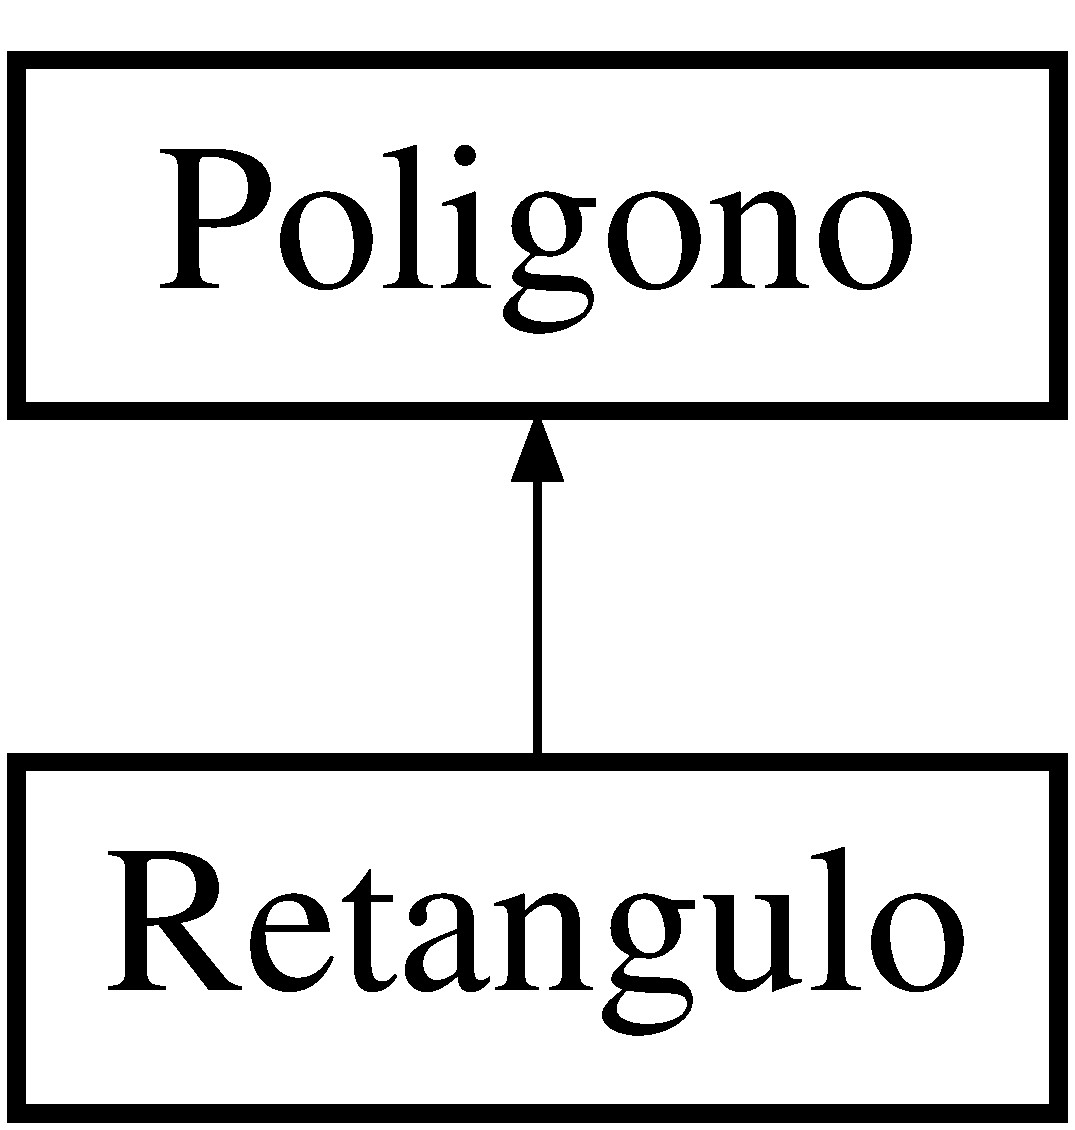
\includegraphics[height=2.000000cm]{class_retangulo}
\end{center}
\end{figure}
\subsection*{Public Member Functions}
\begin{DoxyCompactItemize}
\item 
\mbox{\hyperlink{class_retangulo_acca1dd211eefc8dc04658c943c0d1122}{Retangulo}} (float x, float y, float largura, float altura)
\begin{DoxyCompactList}\small\item\em \mbox{\hyperlink{class_retangulo}{Retangulo}} é um construtor da classe. \end{DoxyCompactList}\end{DoxyCompactItemize}


\subsection{Detailed Description}
A classe \mbox{\hyperlink{class_retangulo}{Retangulo}} serve para representar os pontos do retangulo no espaço bidimensional. 

\subsection{Constructor \& Destructor Documentation}
\mbox{\Hypertarget{class_retangulo_acca1dd211eefc8dc04658c943c0d1122}\label{class_retangulo_acca1dd211eefc8dc04658c943c0d1122}} 
\index{Retangulo@{Retangulo}!Retangulo@{Retangulo}}
\index{Retangulo@{Retangulo}!Retangulo@{Retangulo}}
\subsubsection{\texorpdfstring{Retangulo()}{Retangulo()}}
{\footnotesize\ttfamily Retangulo\+::\+Retangulo (\begin{DoxyParamCaption}\item[{float}]{x,  }\item[{float}]{y,  }\item[{float}]{largura,  }\item[{float}]{altura }\end{DoxyParamCaption})}



\mbox{\hyperlink{class_retangulo}{Retangulo}} é um construtor da classe. 


\begin{DoxyParams}{Parameters}
{\em x,y,largura,altura} & são os valoresatribuido ao póligono. Respectivamente x e y os pontos de origem do retângulo, largura e altura, definem o tamanho do retângulo. \\
\hline
\end{DoxyParams}


The documentation for this class was generated from the following files\+:\begin{DoxyCompactItemize}
\item 
retangulo.\+h\item 
retangulo.\+cpp\end{DoxyCompactItemize}

%--- End generated contents ---

% Index
\backmatter
\newpage
\phantomsection
\clearemptydoublepage
\addcontentsline{toc}{chapter}{Index}
\printindex

\end{document}
